\documentclass{article}
\usepackage{blindtext}
\usepackage{hyperref}
\usepackage{multicol}
\usepackage{graphicx}
\usepackage{float}

\title{Customer Segmentation Clustering based on Demographics and Behaviors}
\author{Spencer Hirsch}
\date{\today}


\begin{document}
\maketitle

% In place of Homework 4, the instructions for the Project 2 report will be changed. The report is required to be written like an academic paper. A minimal outline is:

% - An abstract summarizing your work in <350 words
% - An introduction section with discussion of at least 5 published papers related to your efforts
% - A methods section discussing your preprocessing and models
% - A results section discussing your experiments, model tuning, and performance comparison of models you used
% - A conclusion including your main findings

\begin{multicols}{2}
\section{Abstract}

Identifying similaries between customers can be a useful strategy for companies when creating marketing campaigns. By analyzing the 
demographics and the purchasing behaviors of customers, a company can gain better insight into their customer base.
With valuable insight there is potential to release marketing campaigns targeted towards these groups to increase sales.
By employing unsupervised machine learning we can better identify the characteristics of similar groups to aid in
such campaigns. This study aims to utilize customer demographic and purchasing behaviors to identify trends and group consumers
together based on these characteristics. Through the use of three different unsupervised machine learning clustering methods 
we can identify groups with shared characteristics and attempt to optimize these groups with a variety of preprocessing and 
feature reduction methods to increase the effectiveness of these models in an attempt to find the most effective model for this
study.

\section{Introduction}



\section{Methods}

\begin{table*}
    \centering
    % \resizebox{\columnwidth}{!}{%
        \begin{tabular}{|c|c|}
        % \begin{tabular}{|p{0.3\columnwidth}|p{0.6\columnwidth}|}
            \hline
            \textbf{Feature Name} & \textbf{Feature Description} \\
            \hline
            Id & Unique customer identifier. \\
            Year\_Birth & Birth year of customer. \\
            Education & Highest level of education obtained by customer. \\
            Marital\_Status & Marital status of customer. \\
            Income & Annual income of customer. \\
            Kidhome & Number of young children in the home. \\
            Teenhome & Number of teenagers in the home. \\
            Dt\_Customer & Date when customer first enrolled. \\
            Recency & Last visit of customer. \\
            MntWines & Amount spent on wines. \\
            MntFruits & Amount spent on fruits. \\
            MntMeatProducts & Amount spent on meats. \\
            MntFishProducts & Amount spent on fish. \\
            MntSweetProducts & Amount spent on sweets. \\
            MntGoldProds & Amount spent on gold products. \\
            NumDealsPurchases & Number of purchases made as part of a discount promotion. \\
            NumWebPurchases & Number of purchases made through website. \\
            NumCatalogPurchases & Number of purchases made through catalog \\
            NumStorePurchases & Number of purchases made in store. \\
            NumWebVisitsMonth & Number of times customer has visited the website. \\
            \hline
        \end{tabular}%
    % }
    \caption{Original columns in dataset after removing marketing campaign information.}
\end{table*}

% \subsection{Data Features}
% \begin{table*}
%     \centering
%     \begin{tabular}{|c|c|}
%         \hline
%         \textbf{Feature Name} & \textbf{Feature Description} \\
%         \hline
%         Id & Unique customer identifier. \\
%         Year\_Birth & Birth year of customer. \\
%         Education & Highest level of education obtained by customer. \\
%         Marital\_Status & Marital status of customer. \\
%         Income & Annual income of customer. \\
%         Kidhome & Number of young children in the home. \\
%         Teenhome & Number of teenagers in the home. \\
%         Dt\_Customer & Date when customer first enrolled. \\
%         Recency & Last visit of customer. \\
%         MntWines & Amount spent on wines. \\
%         MntFruits & Amount spent on fruits. \\
%         MntMeatProducts & Amount spent on meats. \\
%         MntFishProducts & Amount spent on fish. \\
%         MntSweetProducts & Amount spent on sweets. \\
%         MntGoldProds & Amount spent on gold products. \\
%         NumDealsPurchases & Number of purchases made as part of a discount promotion. \\
%         NumWebPurchases & Number of purchases made through website. \\
%         NumCatalogPurchases & Number of purchases made through catalog \\
%         NumStorePurchases & Number of purchases made in store. \\
%         NumWebVisitsMonth & Number of times customer has visited the website. \\
%         \hline
%     \end{tabular}
% \end{table*}





In order to prepare the data for this exploration, it was necessary to clean up the data to adhere to the task at hand.
Due to the nature of the project it was fitting that marketing campaign was removed from the dataset, the initial dataset contained 5 marketing campaigns as well as response information from the customers. For the prupose of clustering based on demographic and behaviors this information was not necessarily important.
 
In addition to this feature removal, much of the existing data in the dataset was categorical, rather than leaving objects
in the dataframe, the data was converted to contain only numeric values, this process included 1-hot encoding all categorical
data and splitting the datetime object into three new features, month, day, and year. Following the manual deletion and modification
of the original dataset, the new dataset consisted of 33 features.

\subsection{Preprocessing}

After manual feature reduction and cleaning was performed, additional preprocessing was done on the data. This included utilizing
a variety of methods: Standard Scaler, Robust Scaler, Quantile Transform, and Log Transform. All of these methods were used 
in an attempt to increase the effectiveness of the clusters. We can see that some of the preprocessing methods formed stonger clusters than others. Robust Scaler, seen in figure two, was the worst preprocessing used when it came to clustering. The method that had the strongest clustering was the preprocessing performed with Quantile Transformation, seen in Figure 3.

\begin{figure}[H]
    \centering
    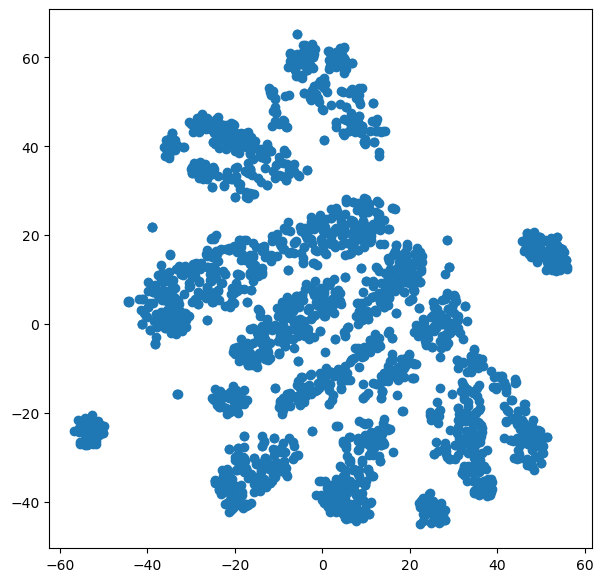
\includegraphics[width=0.4\textwidth]{images/standard_scaler.png}
    \caption{Visual representation of data preprocessed using Standard Scaler.}
\end{figure}

\begin{figure}[H]
    \centering
    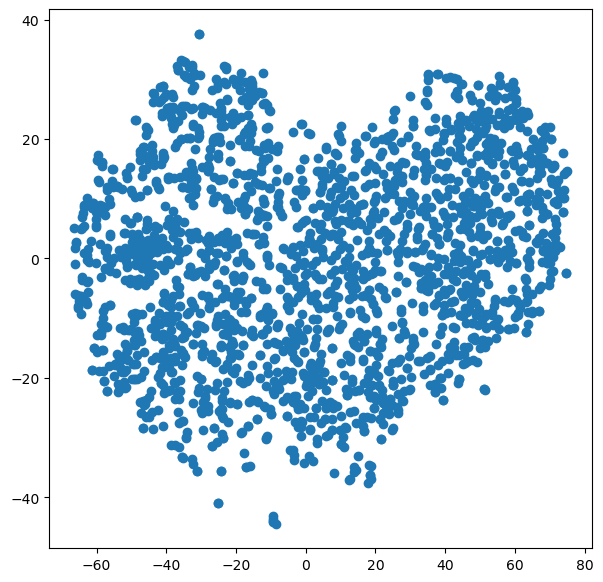
\includegraphics[width=0.4\textwidth]{images/robust_scaler.png}
    \caption{Visual representation of data preprocessed using Robust Scaler.}
\end{figure}

\begin{figure}[H]
    \centering
    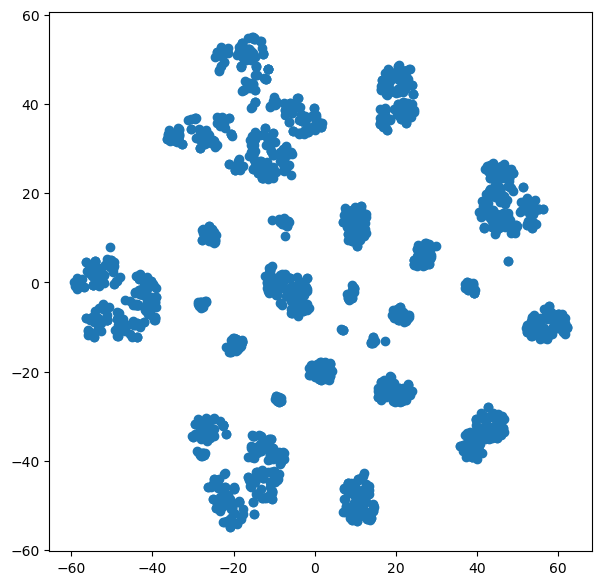
\includegraphics[width=0.4\textwidth]{images/quantile_transform.png}
    \caption{Visual representation of data preprocessed using Quantile Transform.}
\end{figure}

\begin{figure}[H]
    \centering
    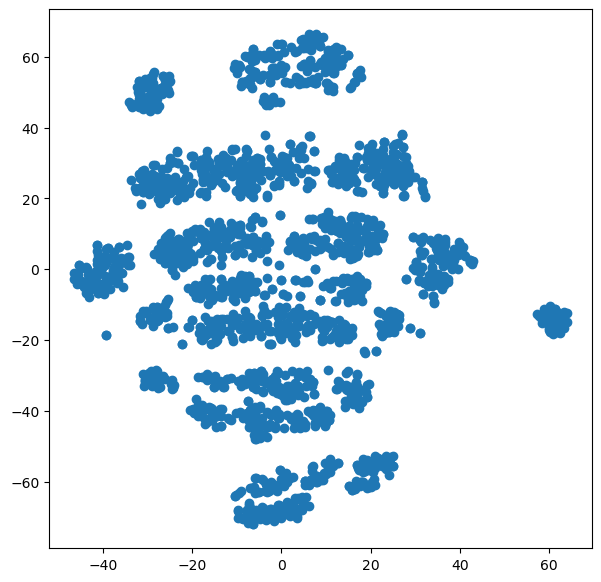
\includegraphics[width=0.4\textwidth]{images/log_transformed.png}
    \caption{Visual representation of data preprocessed using Log Transformed.}
\end{figure}

\subsection{Feature Reduction}

After the dataset had gone through manual reduction

\begin{figure}[H]
    \centering
    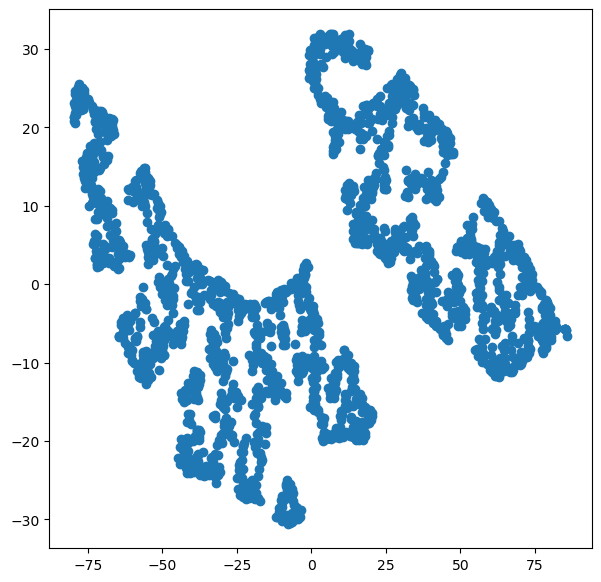
\includegraphics[width=0.4\textwidth]{images/tsne_2.png}
    \caption{Visual representation of data with t-SNE feature reduction with 2 n\_clusters.}
\end{figure}

\begin{figure}[H]
    \centering
    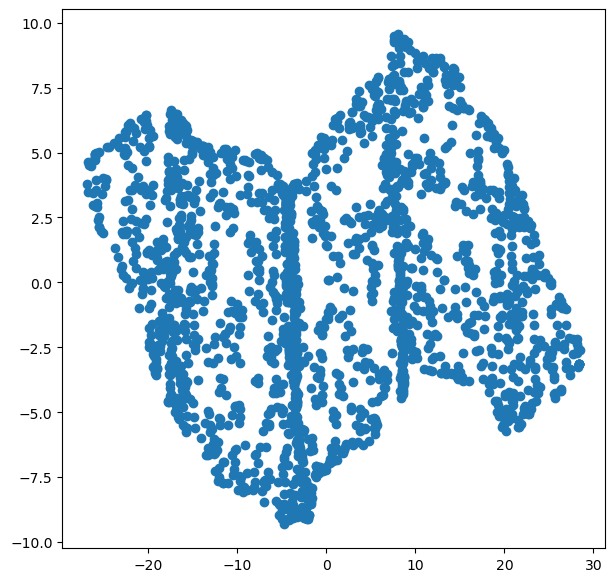
\includegraphics[width=0.4\textwidth]{images/tsne_3.png}
    \caption{Visual representation of data with t-SNE feature reduction with 3 n\_clusters.}
\end{figure}

\subsection{Clustering}

\subsubsection{K-Means}

\begin{figure}[H]
    \centering
    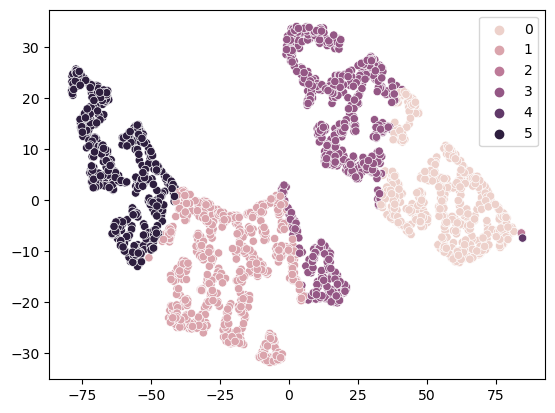
\includegraphics[width=0.4\textwidth]{images/kmeans.png}
    \caption{Visual representation of dataset clustered with K-Means method with t-SNE feature reduction applied.}
\end{figure}

\subsubsection{Hierarchical}

\begin{figure}[H]
    \centering
    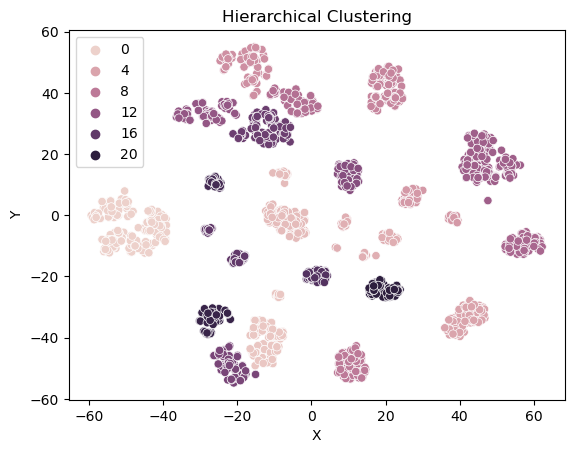
\includegraphics[width=0.4\textwidth]{images/hierarchical.png}
    \caption{Visual representation of dataset clustered with Hierarchical method with t-SNE feature reduction and Quantile Transformation applied.}
\end{figure}

\subsubsection{DBSCAN}

\begin{figure}[H]
    \centering
    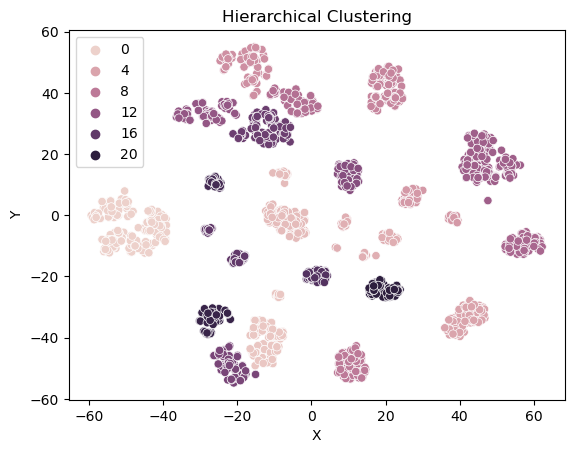
\includegraphics[width=0.4\textwidth]{images/hierarchical.png}
    \caption{Visual representation of dataset clustered with DBSCAN method with t-SNE feature reduction and Quantile Transformation applied.}
\end{figure}
\section{Results}
\section{Conclusion}
\end{multicols}

\pagebreak

% \section{References}

\begin{thebibliography}{9}
    \bibitem{patel_customer_segmentation}
    Patel, Vishakh. \emph{Customer Segmentation/Clustering}. Kaggle. Accessed on April 22, 2024. Available online: \url{https://www.kaggle.com/datasets/vishakhdapat/customer-segmentation-clustering/data}

    \bibitem{zhao_kmeans}
    Zhao, J. (2024). Customer segmentation application based on K-Means. \emph{Applied and Computational Engineering, 47}, 242-247. \url{https://doi.org/10.54254/2755-2721/47/20241400}

    \bibitem{hua}
    Hua, N., Leu, B. A., \& Kumar, R. (2022). Machine learning-based customer segmentation. International Journal of Information Security, 9.

    \bibitem{john}
    John, Jeen \& Shobayo, Olamilekan \& Ogunleye, Bayode. (2023). An Exploration of Clustering Algorithms for Customer Segmentation in the UK Retail Market. Analytics. 2. 809-823. 10.3390/analytics2040042. 

    \bibitem{alie}
    Alie, Juhaini \& Gustriansyah, Rendra. (2024). Customer Segmentation for Digital Marketing Based on Shopping Patterns. Jurnal Aplikasi Bisnis dan Manajemen. 10. 209-216. 10.17358/jabm.10.1.209. 

    \bibitem{li}
    Li, Xiaotong \& Lee, Young. (2024). Customer Segmentation Marketing Strategy Based on Big Data Analysis and Clustering Algorithm. Journal of Cases on Information Technology. 26. 1-16. 10.4018/JCIT.336916. 

\end{thebibliography}

% Patel, Vishakh. "Customer Segmentation/Clustering." Kaggle, n.d., \href{https://www.kaggle.com/datasets/vishakhdapat/customer-segmentation-clustering/data}{}.



\end{document}